
% Estilos TikZ para partículas y líneas
\tikzset{
    particle/.style={circle, fill=black, inner sep=1.5pt, outer sep=2pt},
    label_node/.style={font=\bfseries\small},
    charge_line/.style={blue!60, thick},      % Líneas diagonales (Carga Q)
    strange_line/.style={red!60, thick, dashed}, % Líneas horizontales (Extrañeza S)
    axis_label/.style={font=\tiny\itshape}
}


\hypertarget{Mesones}{\section*{Octete de Mesones ($J^P=0^-$)}}


{
\centering
% --- DIAGRAMA 1: OCTETE DE MESONES (J^P = 0^-) ---
\begin{tikzpicture}[scale=0.75]
    % Coordenadas (Eje X = I3 * 2, Eje Y = S * 1.5)
    \coordinate (K0) at (-1, 1.5);   % S=1, I3=-1/2
    \coordinate (Kp) at (1, 1.5);    % S=1, I3=1/2
    \coordinate (pim) at (-2, 0);    % S=0, I3=-1
    \coordinate (pi0) at (0, 0);     % S=0, I3=0
    \coordinate (pip) at (2, 0);     % S=0, I3=1
    \coordinate (Km) at (-1, -1.5);  % S=-1, I3=-1/2
    \coordinate (K0b) at (1, -1.5);  % S=-1, I3=1/2

    % Líneas de Estructura (Hexágono)
    \draw[thick] (K0) -- (Kp) -- (pip) -- (K0b) -- (Km) -- (pim) -- cycle;

    % Líneas de Carga Q (Azul)
    \draw[charge_line] ($(pim)+(-0.5,0.75)$) -- ($(Km)+(0.5,-0.75)$) node[below] {\tiny $Q=-1$};
    \draw[charge_line] ($(K0)+(-0.5,0.75)$) -- ($(K0b)+(0.5,-0.75)$) node[below] {\tiny $Q=0$};
    \draw[charge_line] ($(Kp)+(-0.5,0.75)$) -- ($(pip)+(0.5,-0.75)$) node[below] {\tiny $Q=+1$};

    % Líneas de Extrañeza S (Rojo)
    \draw[strange_line] (-2.2, 1.5) node[left] {\color{red} $S=+1$} -- (2.2, 1.5);
    \draw[strange_line] (-2.75, 0) node[left] {\color{red} $S=0$} -- (2.5, 0);
    \draw[strange_line] (-2.2, -1.5) node[left] {\color{red} $S=-1$} -- (2.2, -1.5);

    % Partículas
    \node[particle] at (K0) {}; \node[above right] at (K0) {$K^0$};
    \node[particle] at (Kp) {}; \node[above right] at (Kp) {$K^+$};
    \node[particle] at (pim) {}; \node[above left] at (pim) {$\pi^-$};
    \node[particle] at (pi0) {}; \node[above right] at (pi0) {$\pi^0$};
    \node[particle] at (0, -0.3) {}; \node[below left] at (0, -0.3) {$\eta^0$};
    \node[particle] at (pip) {}; \node[above right] at (pip) {$\pi^+$};
    \node[particle] at (Km) {}; \node[below left] at (Km) {$K^-$};
    \node[particle] at (K0b) {}; \node[below left] at (K0b) {$\overline{K}^0$};

\end{tikzpicture}

}

{\section*{Octete de Mesones ($J^P=1^-$)}}

{
\centering
% --- DIAGRAMA 1: OCTETE DE MESONES (J^P = 1^-) ---
\begin{tikzpicture}[scale=0.75]
    % Coordenadas (Eje X = I3 * 2, Eje Y = S * 1.5)
    \coordinate (K0) at (-1, 1.5);   % S=1, I3=-1/2
    \coordinate (Kp) at (1, 1.5);    % S=1, I3=1/2
    \coordinate (pim) at (-2, 0);    % S=0, I3=-1
    \coordinate (pi0) at (0, 0);     % S=0, I3=0
    \coordinate (pip) at (2, 0);     % S=0, I3=1
    \coordinate (Km) at (-1, -1.5);  % S=-1, I3=-1/2
    \coordinate (K0b) at (1, -1.5);  % S=-1, I3=1/2

    % Líneas de Estructura (Hexágono)
    \draw[thick] (K0) -- (Kp) -- (pip) -- (K0b) -- (Km) -- (pim) -- cycle;

    % Líneas de Carga Q (Azul)
    \draw[charge_line] ($(pim)+(-0.5,0.75)$) -- ($(Km)+(0.5,-0.75)$) node[below] {\tiny $Q=-1$};
    \draw[charge_line] ($(K0)+(-0.5,0.75)$) -- ($(K0b)+(0.5,-0.75)$) node[below] {\tiny $Q=0$};
    \draw[charge_line] ($(Kp)+(-0.5,0.75)$) -- ($(pip)+(0.5,-0.75)$) node[below] {\tiny $Q=+1$};

    % Líneas de Extrañeza S (Rojo)
    \draw[strange_line] (-2.2, 1.5) node[left] {\color{red} $S=+1$} -- (2.2, 1.5);
    \draw[strange_line] (-2.75, 0) node[left] {\color{red} $S=0$} -- (2.5, 0);
    \draw[strange_line] (-2.2, -1.5) node[left] {\color{red} $S=-1$} -- (2.2, -1.5);

    % Partículas
    \node[particle] at (K0) {}; \node[above right] at (K0) {$K^{*0}$};
    \node[particle] at (Kp) {}; \node[above right] at (Kp) {$K^{*+}$};
    \node[particle] at (pim) {}; \node[above left] at (pim) {$\rho^-$};
    \node[particle] at (pi0) {}; \node[above right] at (pi0) {$\rho^0$};
    \node[particle] at (0, -0.3) {}; \node[below left] at (0, -0.3) {$\omega^0$};
    \node[particle] at (pip) {}; \node[above right] at (pip) {$\rho^+$};
    \node[particle] at (Km) {}; \node[below left] at (Km) {$K^{*-}$};
    \node[particle] at (K0b) {}; \node[below left] at (K0b) {$\overline{K}^{*0}$};

\end{tikzpicture}

}

% --- DIAGRAMA 2: OCTETE DE BARIONES (J^P = 1/2^+) ---
\hypertarget{Bariones}{\section*{Octete de Bariones ($J^P=1/2^+$)}}

{
\centering
\begin{tikzpicture}[scale=0.75]
    % Coordenadas
    \coordinate (n) at (-1, 1.5);    % S=0, I3=-1/2
    \coordinate (p) at (1, 1.5);     % S=0, I3=1/2
    \coordinate (Sm) at (-2, 0);     % S=-1, I3=-1
    \coordinate (S0) at (0, 0);      % S=-1, I3=0
    \coordinate (Sp) at (2, 0);      % S=-1, I3=1
    \coordinate (Xm) at (-1, -1.5);  % S=-2, I3=-1/2
    \coordinate (X0) at (1, -1.5);   % S=-2, I3=1/2

    % Hexágono
    \draw[thick] (n) -- (p) -- (Sp) -- (X0) -- (Xm) -- (Sm) -- cycle;

    % Líneas Q
    \draw[charge_line] ($(Sm)+(-0.5,0.75)$) -- ($(Xm)+(0.5,-0.75)$) node[below] {\tiny $Q=-1$};
    \draw[charge_line] ($(n)+(-0.5,0.75)$) -- ($(X0)+(0.5,-0.75)$) node[below] {\tiny $Q=0$};
    \draw[charge_line] ($(p)+(-0.5,0.75)$) -- ($(Sp)+(0.5,-0.75)$) node[below] {\tiny $Q=+1$};

    % Líneas S
    \draw[strange_line] (-2.2, 1.5) node[left] {\color{red} $S=0$} -- (2.2, 1.5);
    \draw[strange_line] (-2.75, 0) node[left] {\color{red} $S=-1$} -- (2.5, 0);
    \draw[strange_line] (-2.2, -1.5) node[left] {\color{red} $S=-2$} -- (2.2, -1.5);

    % Partículas
    \node[particle] at (n) {}; \node[above right] at (n) {$n$};
    \node[particle] at (p) {}; \node[above right] at (p) {$p$};
    \node[particle] at (Sm) {}; \node[above left] at (Sm) {$\Sigma^-$};
    \node[particle] at (S0) {}; \node[above right] at (S0) {$\Sigma^0$};
    \node[particle] at (0, -0.3) {}; \node[below left] at (0, -0.3) {$\Lambda$};
    \node[particle] at (Sp) {}; \node[above right] at (Sp) {$\Sigma^+$};
    \node[particle] at (Xm) {}; \node[below left] at (Xm) {$\Xi^-$};
    \node[particle] at (X0) {}; \node[below left] at (X0) {$\Xi^0$};

\end{tikzpicture}

}

% --- DIAGRAMA 3: DECUPLETE DE BARIONES (J^P = 3/2^+) ---
\hypertarget{Bariones_big}{\section*{Decuplete de Bariones ($J^P=3/2^+$)}}

{
\centering
\begin{tikzpicture}[scale=0.6]
    % Coordenadas (Triángulo Invertido)
    % Fila S=0 (Deltas)
    \coordinate (Dmm) at (-3, 2.25); % I3=-3/2
    \coordinate (Dm) at (-1, 2.25);  % I3=-1/2
    \coordinate (D0) at (1, 2.25);   % I3=1/2
    \coordinate (Dp) at (3, 2.25);   % I3=3/2
    
    % Fila S=-1 (Sigmas*)
    \coordinate (Sms) at (-2, 0.75); % I3=-1
    \coordinate (S0s) at (0, 0.75);  % I3=0
    \coordinate (Sps) at (2, 0.75);  % I3=1
    
    % Fila S=-2 (Xi*)
    \coordinate (Xms) at (-1, -0.75);% I3=-1/2
    \coordinate (X0s) at (1, -0.75); % I3=1/2
    
    % Fila S=-3 (Omega)
    \coordinate (Om) at (0, -2.25);  % I3=0

    % Estructura
    \draw[thick] (Dmm) -- (Dp) -- (Om) -- cycle;

    % Definición del vector director base
    \coordinate (Start_Q_minus1) at ($(Dmm)+(-0.60,0.95)$);
    \path let \p1 = ($(Om)-(Start_Q_minus1)$) in coordinate (vec) at (\x1,\y1);
    
    % --- Q = -1 ---
    % Escalar 1.1 ANTES del vector
    \draw[charge_line] (Start_Q_minus1) -- ++($ 1.1*(vec) $) 
        node[right] {\tiny $Q=-1$};
    
    % --- Q = 0 ---
    \draw[charge_line] ($(Dm)+(-0.5,0.75)$) -- ++($ 0.8*(vec) $) 
        node[right, xshift=5pt] {\tiny $Q=0$};
    
    % --- Q = 1 ---
    \draw[charge_line] (0.55,3) -- ++($ 0.50*(vec) $) 
        node[right, xshift=5pt] {\tiny $Q=1$};
    
    % --- Q = 2 ---
    \draw[charge_line] (2.5,3) -- ++($ 0.3*(vec) $) 
        node[right, xshift=5pt] {\tiny $Q=2$};
    
    % Líneas S
    \draw[strange_line] (-3.5, 2.25) node[left] {\color{red} $S=0$} -- (3.5, 2.25);
    \draw[strange_line] (-2.95, 0.75) node[left] {\color{red} $S=-1$} -- (2.5, 0.75);
    \draw[strange_line] (-1.95, -0.75) node[left] {\color{red} $S=-2$} -- (1.5, -0.75);
    \draw[strange_line] (-0.5, -2.25) node[left] {\color{red} $S=-3$} -- (0.5, -2.25);

    % Partículas
    \node[particle] at (Dmm) {}; \node[above right] at (Dmm) {$\Delta^-$};
    \node[particle] at (Dm) {}; \node[above right] at (Dm) {$\Delta^0$};
    \node[particle] at (D0) {}; \node[above right] at (D0) {$\Delta^+$};
    \node[particle] at (Dp) {}; \node[above right] at (Dp) {$\Delta^{++}$};
    
    \node[particle] at (Sms) {}; \node[above left] at (Sms) {$\Sigma^{*-}$};
    \node[particle] at (S0s) {}; \node[above right] at (S0s) {$\Sigma^{*0}$};
    \node[particle] at (Sps) {}; \node[above right] at (Sps) {$\Sigma^{*+}$};
    
    \node[particle] at (Xms) {}; \node[above left] at (Xms) {$\Xi^{*-}$};
    \node[particle] at (X0s) {}; \node[above right] at (X0s) {$\Xi^{*0}$};
    
    \node[particle] at (Om) {}; \node[below left] at (Om) {$\Omega^-$};

\end{tikzpicture}

}

\hypertarget{Gluones}{\section*{Octuplete de Gluones}}


{
\centering
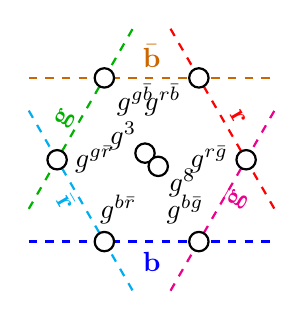
\begin{tikzpicture}[scale=1.2, >=latex]
    % Definición de coordenadas
    \coordinate (Center) at (0,0);
    \coordinate (Gr) at (-1, 0);       % g^{g \bar{r}}
    \coordinate (Rg) at (1, 0);        % g^{r \bar{g}}
    \coordinate (Gb) at (-0.5, 0.866); % g^{g \bar{b}}
    \coordinate (Rb) at (0.5, 0.866);  % g^{r \bar{b}}
    \coordinate (Br) at (-0.5, -0.866);% g^{b \bar{r}}
    \coordinate (Bg) at (0.5, -0.866); % g^{b \bar{g}}

    % --- LÍNEAS DE FLUJO DE COLOR (Ejes Discontinuos) ---
    % Los colores se han ajustado para coincidir con la imagen proporcionada

    % 1. Ejes Horizontales
    % Anti-blue (Naranja)
    \draw[dashed, color=orange!80!black, thick] (-1.3, 0.866) -- (1.3, 0.866) 
        node[midway, above, font=\bfseries] {$\bar{\textbf{b}}$};
    % Blue (Azul)
    \draw[dashed, color=blue, thick] (-1.3, -0.866) -- (1.3, -0.866) 
        node[midway, below, font=\bfseries] {b};

    % 2. Ejes Diagonales \ (Verde / Magenta)
    % Green (Verde)
    \draw[dashed, color=green!70!black, thick] (-1.3, -0.52) -- (-0.2, 1.386) 
        node[pos=0.75, left, rotate=60, font=\bfseries, xshift = -15pt, yshift=5pt] {g};
    % Anti-green (Magenta)
    \draw[dashed, color=magenta, thick] (0.2, -1.386) -- (1.3, 0.52) 
        node[pos=0.25, right, rotate=60, font=\bfseries, xshift=15pt, yshift=-4pt] {$\bar{\textbf{g}}$};

    % 3. Ejes Diagonales / (Cian / Rojo)
    % Anti-red (Cian)
    \draw[dashed, color=cyan, thick] (-1.3, 0.52) -- (-0.2, -1.386) 
        node[pos=0.75, left, rotate=-60, font=\bfseries, xshift=-15pt,yshift=-5pt] {$\bar{\textbf{r}}$};
    % Red (Rojo)
    \draw[dashed, color=red, thick] (0.2, 1.386) -- (1.3, -0.52) 
        node[pos=0.25, right, rotate=-60, font=\bfseries, xshift=15, yshift=5pt] {r};

    % --- NODOS (Partículas) ---
    % Círculos más grandes con borde grueso
    \tikzset{gluon/.style={fill=white, draw=black, thick, circle, minimum size=7pt, inner sep=0pt}}

    \node[gluon] at (Gr) {};
    \node[gluon] at (Rg) {};
    \node[gluon] at (Gb) {};
    \node[gluon] at (Rb) {};
    \node[gluon] at (Br) {};
    \node[gluon] at (Bg) {};

    % Nodo central doble
    \node[gluon] at (-0.07, 0.07) {};
    \node[gluon] at (0.07, -0.07) {};

    % --- ETIQUETAS (Estados de los gluones) ---
    % Posiciones ajustadas para coincidir con la imagen
    \node[right, xshift=1pt, yshift = -8pt] at (Gb) {$g^{g\bar{b}}$};
    \node[left, xshift=-3pt, yshift = -8pt] at (Rb) {$g^{r\bar{b}}$};
    \node[right, xshift=3pt] at (Gr) {$g^{g\bar{r}}$};
    \node[left, xshift=-3pt] at (Rg) {$g^{r\bar{g}}$};
    \node[above, xshift = 5pt, yshift=3pt] at (Br) {$g^{b\bar{r}}$};
    \node[above, xshift=-5pt, yshift=3pt] at (Bg) {$g^{b\bar{g}}$};

    % Etiquetas centrales
    \node[left, xshift=-2pt] at (0, 0.25) {$g^3$};
    \node[right, xshift=2pt] at (0.02, -0.25) {$g^8$};

\end{tikzpicture}


}

